\documentclass{beamer}

\usepackage{booktabs}
\usepackage{multirow}
\usepackage{array}
\usepackage{graphicx}
\usepackage[table]{xcolor}
\usepackage{animate}

\usepackage{tikz}
\usepackage{opensans}
\usepackage[T1]{fontenc}
\usepackage{fix-cm}
\usetikzlibrary{shapes.geometric, positioning, calc}

\renewcommand{\familydefault}{\sfdefault}

\usetheme{default}
\usecolortheme{rose}
\setbeamertemplate{navigation symbols}{}
\setbeamercolor{title}{fg=red!80!black}
\setbeamercolor{author}{fg=gray!40!black}
\setbeamercolor{frametitle}{fg=gray!20!black}

\newcommand{\veryHuge}{\fontsize{40}{48}\selectfont}

\newcommand{\subjectPresentation}[3]{ % section nb, section name, section color
  \begin{frame}
    \frametitle{}
    \centering
    \begin{tikzpicture}
      \node[diamond, draw=gray!50, line width=8pt, fill=none, minimum size=6cm] (n) 
            {\veryHuge\textcolor{#3}{\textbf{#1}}};
      \node[below=-1.2cm of n, rectangle, fill=white, minimum width=5cm, 
            minimum height=1cm, anchor=center, text=#3, 
            font=\LARGE\bfseries] {#2};
    \end{tikzpicture}
    \begin{tikzpicture}[overlay,remember picture]
      \fill[#3] (current page.south west) -- 
            (current page.north west) -- 
            ([xshift=0.3\paperwidth]current page.south west) -- cycle;
    \end{tikzpicture}
  \end{frame}
}

\newcommand{\subjectDevelopment}[3]{ % title, text, color
  \begin{frame}
    \frametitle{#1}
    #2
    \begin{tikzpicture}[overlay,remember picture]
      \fill[#3!50!white] (current page.west) -- 
            ([yshift=0.7cm]current page.west) -- 
            ([xshift=0.7cm]current page.west) -- 
            ([yshift=-0.7cm]current page.west) -- cycle;
    \end{tikzpicture}
  \end{frame}
}

\definecolor{color1}{RGB}{54, 69, 255} % blue
\definecolor{color2}{RGB}{94,23,235} % purple
\definecolor{color3}{RGB}{12, 192, 223} % cyan
\definecolor{color4}{RGB}{193, 114, 80} % brown
\definecolor{color5}{RGB}{143, 220, 187} % green
\definecolor{color6}{RGB}{195, 63, 54} % red

\title{Explainability of high-dimensional prediction models using neural networks}
\author{DE QUEIROZ GARCIA, Luana}

\addtobeamertemplate{footline}{
  \ifnum\thepage>1
    \begin{tikzpicture}[overlay,remember picture]
      \node[anchor=south east] at (current page.south east) {
        
\includegraphics[width=3cm]{Images/logo_ensta.png}
      };
    \end{tikzpicture}
  \fi
}{}

\begin{document}

\begin{frame}[plain]
  \begin{tikzpicture}[remember picture,overlay]
    \node at (current page){
\includegraphics[height=1\paperheight, keepaspectratio]{Images/background_ensta.png}};
  \end{tikzpicture}
  \vspace*{1cm}
  \centering
  
\includegraphics[width=3cm]{Images/logo_ensta_vert.png}
  
  \vfill
  
  {\usebeamerfont{title}\usebeamercolor[fg]{title}\inserttitle\par}
  \vspace{0.5cm}
  {\usebeamerfont{author}\usebeamercolor[fg]{author}\insertauthor\par}
  
  \vfill
\end{frame}

\begin{frame}
  \frametitle{}
  \centering
  This internship was a result of a partnership between:
  \vfill
  
\includegraphics[width=2cm]{Images/logo_ensta_vert.png}
  \hspace{1cm}
  
\includegraphics[width=3.5cm]{Images/inria_logo.png}
  \vfill
  
\includegraphics[width=3cm]{Images/logo_imt.png}
  \hspace{1cm}
  
\includegraphics[width=2.5cm]{Images/logo_meteo_france.png}
  
\end{frame}

\begin{frame}
    \frametitle{}
    \centering
    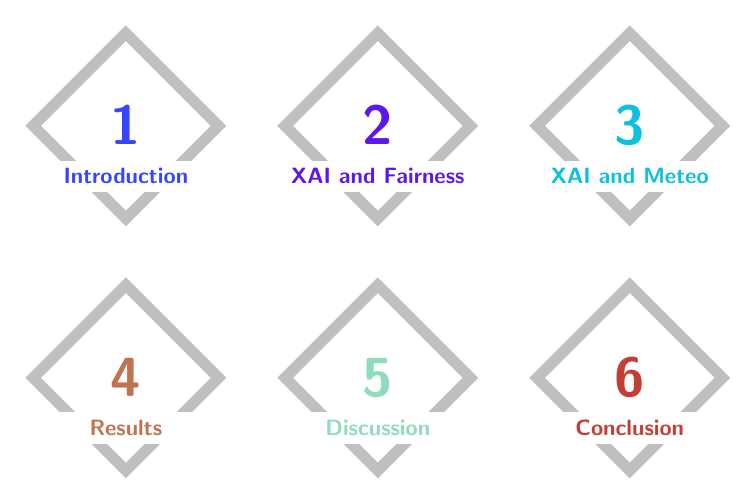
\begin{tikzpicture}[scale=0.8, transform shape]
        % First row
        \foreach \x/\num/\text/\col in {0/1/Introduction/color1, 4/2/XAI and Fairness/color2, 8/3/XAI and Meteo/color3} {
        \node[diamond, draw=gray!50, line width=4pt, fill=none, minimum size=3cm] at (\x,0) {\Huge\textcolor{\col}{\textbf{\num}}};
        \node[below=0.8cm, rectangle, fill=white, minimum width=3cm, 
                minimum height=0.5cm, anchor=center] at (\x,0) {\textcolor{\col}{\bfseries \text}};
        }
        
        % Second row  
        \foreach \x/\num/\text/\col in {0/4/Results/color4, 4/5/Discussion/color5, 8/6/Conclusion/color6} {
        \node[diamond, draw=gray!50, line width=4pt, fill=none, minimum size=3cm] at (\x,-4) {\Huge\textcolor{\col}{\textbf{\num}}};
        \node[below=0.8cm, rectangle, fill=white, minimum width=3cm, 
                minimum height=0.5cm, anchor=center] at (\x,-4) {\textcolor{\col}{\bfseries \text}};
        }
    \end{tikzpicture}
    \begin{tikzpicture}[overlay,remember picture]
        \fill[gray!50] (current page.west) -- 
            ([yshift=1cm]current page.west) -- 
            ([xshift=1cm]current page.west) -- 
            ([yshift=-1cm]current page.west) -- cycle;
    \end{tikzpicture}
\end{frame}

\subjectPresentation{1}{Introduction}{color1}

\subjectDevelopment{Context}{
    \centering
    
\begin{tikzpicture}[node distance=3cm]
        \node[circle, draw, fill=color2!20, minimum size=3cm, align=center, text width=2cm] (a) {Analysis of the \\ USA Census};
        \node[circle, draw, fill=color3!20, minimum size=3cm, align=center, text width=2cm] (b) [right=of a] {Weather\\Forecasting};
    \end{tikzpicture}
    \vfill
    What's the importance of these themes? Why do we use Machine Learning to do these tasks? And how they are linked?
}{color1}

\subjectDevelopment{First subject: The USA Census}{
\begin{columns}[T]
    \begin{column}{0.5\textwidth}

        \begin{itemize}
            \item Data of Analysis: Folktables dataset
            \item Application: Prediction of a person's income (higher and lower income)
            \item \textbf{Objective: Undestand patterns on the population, that can be used by banks (e.g. loan release)}
        \end{itemize}
        
    \end{column}
    \begin{column}{0.5\textwidth}
        \centering
        \scriptsize
        \begin{table}[h]
            \caption{Folktables Features}
            \begin{tabular}{p{1.2cm}p{1.8cm}}
                \hline
                \textbf{Feature} & \textbf{Description} \\
                \hline
                AGEP & Age \\
                COW & Worker Class \\
                SCHL & Education \\
                MAR & Marital Status \\
                OCCP & Occupation \\
                POBP & Birth Place \\
                RELP & Relationship \\
                WKHP & Work Hours \\
                SEX & Sex \\
                RAC1P & Race \\
                \hline
            \end{tabular}
        \end{table}
    \end{column}
\end{columns}
}{color1}

\subjectDevelopment{Second subject: Weather forecasting}{
\begin{columns}[T]
    \begin{column}{0.5\textwidth}
        \begin{itemize}
            \item Data of Analysis: Titan dataset (AROME and ARPÈGE images)
            \item Application: Prediction of the weather (variables of temperature, wind, geopotencial, humidity, ...) in the next hour
            \item \textbf{Objective: 100x Faster weather predictions, less computational resources, investigation of extreme climate events}
        \end{itemize}
    \end{column}

    \begin{column}{0.5\textwidth}
        \centering
        \scriptsize
        
        \begin{figure}[h]
            % Imagens muito pequenas
            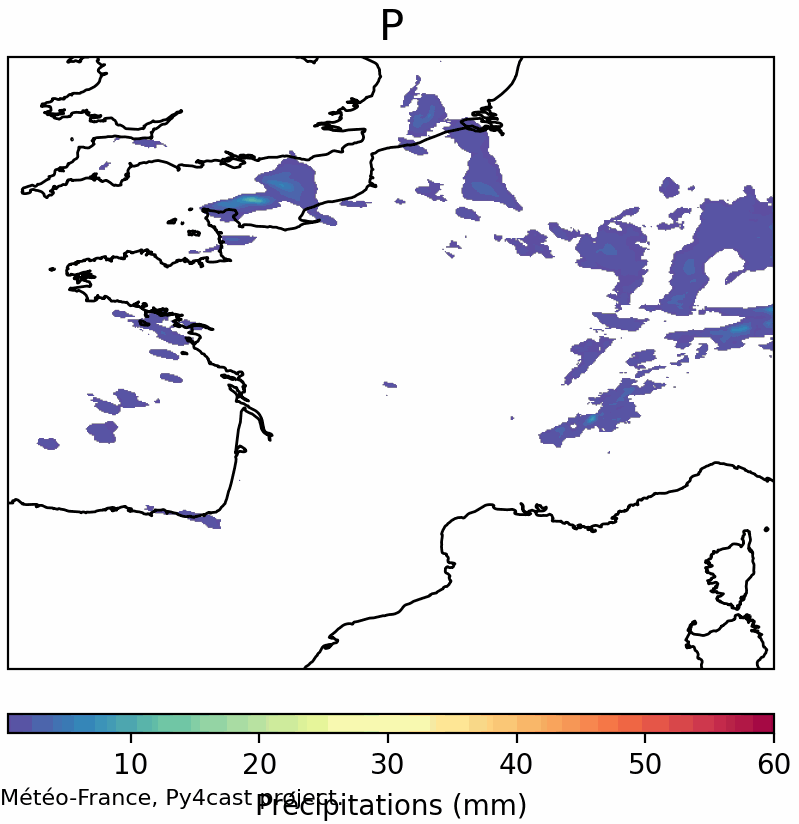
\includegraphics[width=0.4\textwidth]{Images/titan_data_examples/2023111700_feature_aro_tp_0m.png}
            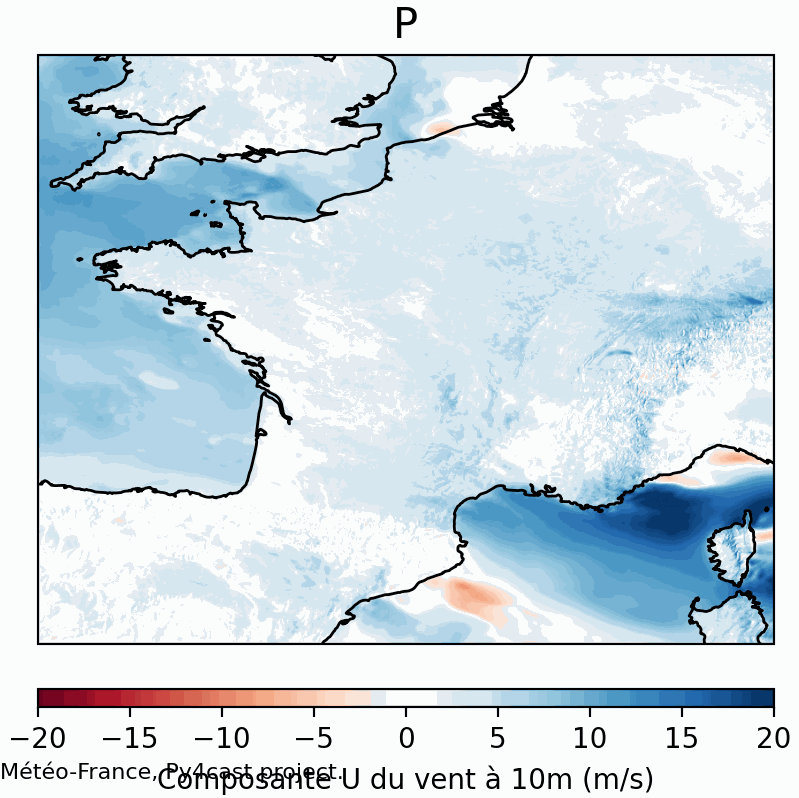
\includegraphics[width=0.4\textwidth]{Images/titan_data_examples/2023111700_feature_aro_u10_10m.png}
            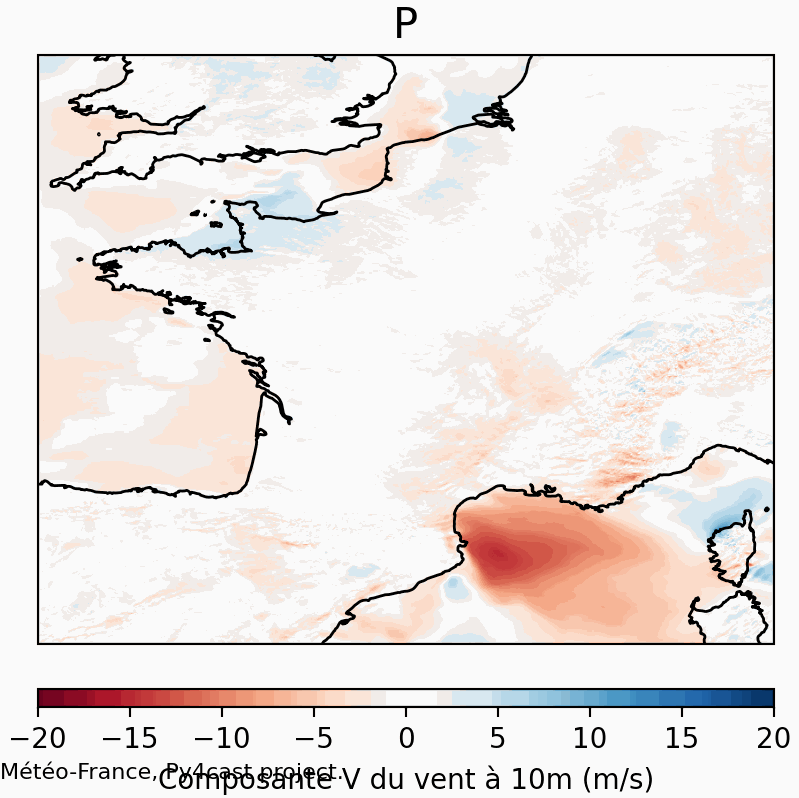
\includegraphics[width=0.4\textwidth]{Images/titan_data_examples/2023111700_feature_aro_v10_10m.png}
            
            \vspace{0.1cm}
            \begin{minipage}{0.4\textwidth}
                \centering\tiny TP 0m
            \end{minipage}
            \hfill
            \begin{minipage}{0.4\textwidth}
                \centering\tiny U10 10m
            \end{minipage}
            \hfill
            \begin{minipage}{0.4\textwidth}
                \centering\tiny V10 10m
            \end{minipage}
            
            \vspace{0.1cm}
            \caption{\scriptsize Titan image channels}
        \end{figure}
    \end{column}
\end{columns}
}{color1}

\subjectDevelopment{What's eXplainable AI (XAI)}{
    The XAI is a domain that gives tools to increase the user's \textbf{interpretability and trust} on the results of Artificial Intelligence (AI) models.

    \vfill

    Critical domains require investigation...

    \vfill

    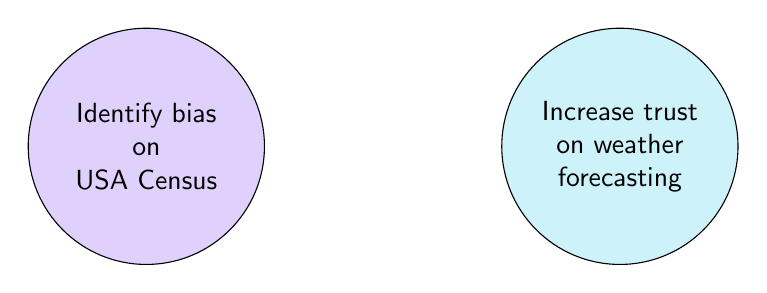
\begin{tikzpicture}[node distance=3cm]
        \node[circle, draw, fill=color2!20, minimum size=3cm, align=center, text width=2cm] (a) {Identify bias \\ on \\ USA Census};
        \node[circle, draw, fill=color3!20, minimum size=3cm, align=center, text width=2cm] (b) [right=of a] {Increase trust \\ on weather \\ forecasting};
    \end{tikzpicture}
}{color1}

\subjectDevelopment{Main ideas explored}{
  \begin{enumerate}
    \item Understanding the results of the AI “black boxes”
    \begin{enumerate}
      \item The need to develop adapted eXplainable AI (XAI) techniques
      \item Verify that the model's results are made with the "right reasons"
    \end{enumerate}
    \item Adaptable XAI techniques (low and high dimensional data)
    \begin{enumerate}
      \item Used for classification and regression tasks
      \item Explanations that are representable
    \end{enumerate}
  \end{enumerate}
}{color1}

\subjectDevelopment{XAI techniques}{
    \begin{itemize}
        \item SHAP, Lime (perturbation-based)
        \item \textbf{Anchors} (example-based)
        \item Smooth Gradient, Integrated Gradient (gradient-based)
    \end{itemize}
}{color1}

\subjectDevelopment{Why exploring Anchors?}{
    \centering
    Explanations with a promise of being compact and representable, other than being a high precision result, and human understandable!

    \vfill

    \textit{More precise for low-dimensional data, and adaptable for high-dimensional data.}
}{color1}

\subjectDevelopment{Diving deeper on Anchors}{
    Considering a binary classifier $f : \mathcal{X} \rightarrow \{0, 1\}$. For a given instance $x$, the objective is to find a predicate \textbf{$A$ that explains the prediction $f(x)$ by identifying a minimal set of decisive features}.

    A predicate $A$ is deemed a valid anchor if it meets a precision threshold, meaning it \textbf{guarantees the model's output is consistent under local perturbation}. Precision is formally defined as:
    \begin{equation}
    \text{prec}(A) = \mathbb{E}_{D(z|A)} [\mathbf{1}_{f(x) = f(z)}]
    \label{eq:prec-anchors}
    \end{equation}
    where $D(\cdot|A)$ is the conditional distribution of inputs satisfying $A$. The anchor condition is satisfied with high confidence if $P(\text{prec}(A) \geq \tau) \geq 1 - \delta$.
}{color1}
\subjectDevelopment{Diving deeper on Anchors}{
    To select the most impactful and parsimonious explanation for end-users, the method introduces a coverage measure. The coverage of \textbf{$A$ is defined as the probability that the predicate holds under the data distribution}:
    \begin{equation}
    \text{cov}(A) = \mathbb{E}_{D(z)} [A(z)]
    \label{eq:cov-anchors}
    \end{equation}

    For a given data distribution $D$, parameters $\tau$ and $\delta$, the optimal anchor is the one with maximum coverage subject to the precision constraint:
    \begin{equation}
    \arg \max_{A} {\text{cov}(A) \mid P(\text{prec}(A) \geq \tau) \geq 1 - \delta }
    \label{eq:max-cov-anchors}
    \end{equation}
}{color1}

\subjectPresentation{2}{XAI for the USA Census}{color2}

\subjectDevelopment{Analyse Fairness on the USA Census}{
	\begin{itemize}
		\item Can we find bias in the ML models?
		\item If so, can we use XAI to identify where's the problem?
	\end{itemize}
	\vfill
	\centering
	We used the 'SEX' as the sensible variable.
}{color2}

\subjectDevelopment{Trained Models}{
\begin{itemize}
	\item \textbf{Logistic Regression}
	
    \item \textbf{XGBoost} (eXtreme Gradient Boosting)
	
	\item \textbf{Hist Gradient Boosting} (Skrub's Scikit-learn implementation)
	
	\item \textbf{Simple Neural Network}
\end{itemize}
}{color2}

\subjectDevelopment{Fairness Metrics}{
\begin{itemize}
	\item \textbf{Accuracy}: The proportion of correct predictions (both true positives and true negatives) among all predictions.

	\item \textbf{Disparate Impact (DI)}: Measures the ratio between the \textbf{proportion of positive outcomes for the protected group (women) versus the privileged group (men)}. Values close to 1 indicate fairness, while values below 1 suggest bias against the protected group.

	\item \textbf{Equality of Odds}: Examines whether both groups have equal true positive rates and equal false positive rates. Values closer to 1 indicate better fairness.

	\item \textbf{Sufficiency}: Assesses whether the probability of the true outcome is the same across groups given the predicted outcome. Values closer to 1 indicate better fairness.
\end{itemize}
}{color2}

\subjectDevelopment{Performance and Fairness metrics}{
\begin{table}[h]
\centering
\caption{Model Performance Comparison Across States (Accuracy and Fairness Metrics)}
\label{tab:folktables-results}
\resizebox{\textwidth}{!}
{
\begin{tabular}{llcccccc}
\toprule
\textbf{Model} & \textbf{Training} & \textbf{Testing} & \textbf{Accuracy} & \textbf{Disparate Impact} & \textbf{Equality of Odds} & \textbf{Sufficiency} \\
\midrule
\rowcolor{gray!10}
\multirow{6}{*}{Logistic Regression} 
& \multirow{2}{*}{CA} & CA & 0.56 & 0.67 & 0.84 & 0.95 \\
& & USA & 0.52 & 0.66 & 0.88 & 0.86 \\
\cmidrule(lr){2-7}
& \multirow{2}{*}{TX} & TX & 0.52 & 0.46 & 0.65 & 0.90 \\
& & USA & 0.51 & 0.46 & 0.67 & 0.95 \\
\cmidrule(lr){2-7}
& \multirow{2}{*}{NY} & NY & 0.51 & 0.66 & 0.82 & 0.93 \\
& & USA & 0.52 & 0.64 & 0.86 & 0.88 \\
\midrule

\rowcolor{gray!10}
\multirow{6}{*}{XGBoost} 
& \multirow{2}{*}{CA} & CA & 0.64 & 0.72 & 0.91 & 0.96 \\
& & USA & 0.58 & 0.67 & 0.92 & 0.90 \\
\cmidrule(lr){2-7}
& \multirow{2}{*}{TX} & TX & 0.60 & 0.58 & 0.83 & 0.93 \\
& & USA & 0.58 & 0.58 & 0.85 & 0.95 \\
\cmidrule(lr){2-7}
& \multirow{2}{*}{NY} & NY & 0.61 & 0.75 & 0.92 & 0.96 \\
& & USA & 0.57 & 0.67 & 0.92 & 0.90 \\
\midrule

\rowcolor{gray!10}
\multirow{6}{*}{HistGradientBoosting} 
& \multirow{2}{*}{CA} & CA & 0.63 & 0.71 & 0.90 & 0.94 \\
& & USA & 0.58 & 0.67 & 0.92 & 0.90 \\
\cmidrule(lr){2-7}
& \multirow{2}{*}{TX} & TX & 0.61 & 0.54 & 0.78 & 0.96 \\
& & USA & 0.58 & 0.56 & 0.83 & 0.97 \\
\cmidrule(lr){2-7}
& \multirow{2}{*}{NY} & NY & 0.60 & 0.68 & 0.89 & 0.97 \\
& & USA & 0.58 & 0.64 & 0.90 & 0.91 \\
\midrule

\rowcolor{gray!10}
\multirow{6}{*}{Neural Network} 
& \multirow{2}{*}{CA} & CA & 0.52 & 0.88 & 1.03 & 0.85 \\
& & USA & 0.46 & 0.65 & 0.86 & 0.86 \\
\cmidrule(lr){2-7}
& \multirow{2}{*}{TX} & TX & 0.50 & 0.61 & 0.87 & 0.94 \\
& & USA & 0.49 & 0.77 & 0.96 & 0.81 \\
\cmidrule(lr){2-7}
& \multirow{2}{*}{NY} & NY & 0.51 & 0.76 & 0.93 & 0.92 \\
& & USA & 0.48 & 0.66 & 0.88 & 0.87 \\
\bottomrule
\end{tabular}%
}
\end{table}
}{color2}

\subjectDevelopment{Applying Anchors}{
Our focus is on Meteo today, so it's just important to know that our results found zones in the population with high indication of unfairness.
}{color2}

\subjectPresentation{3}{XAI and Meteo}{color3}

\subjectDevelopment{Analyse truthfulness of Results}{
	\begin{itemize}
		\item Can we explain the ML models decisions on a human understandable way?
		\item If so, can we use XAI to identify relations between regions, how they influence each other?
	\end{itemize}
	\vfill
	\centering
	We used the Titan data from November 2023 and the UNetR++ convolutional neural network 
}{color3}

\subjectDevelopment{The Titan data}{
    21 channels of AROME images + 16 channels of ARPÈGE images
    \vfill
    \begin{figure}[h]
        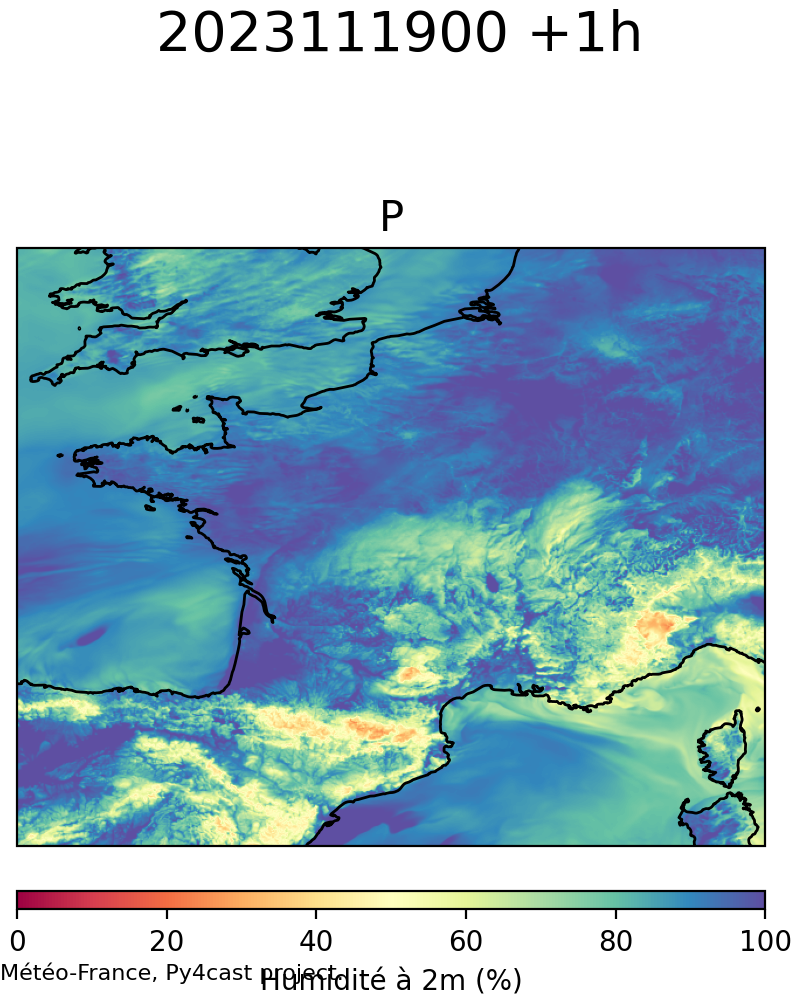
\includegraphics[width=0.2\textwidth]{Images/titan_data_examples/19_11/2023111900_feature_aro_r2_2m.png}
        \hfill
        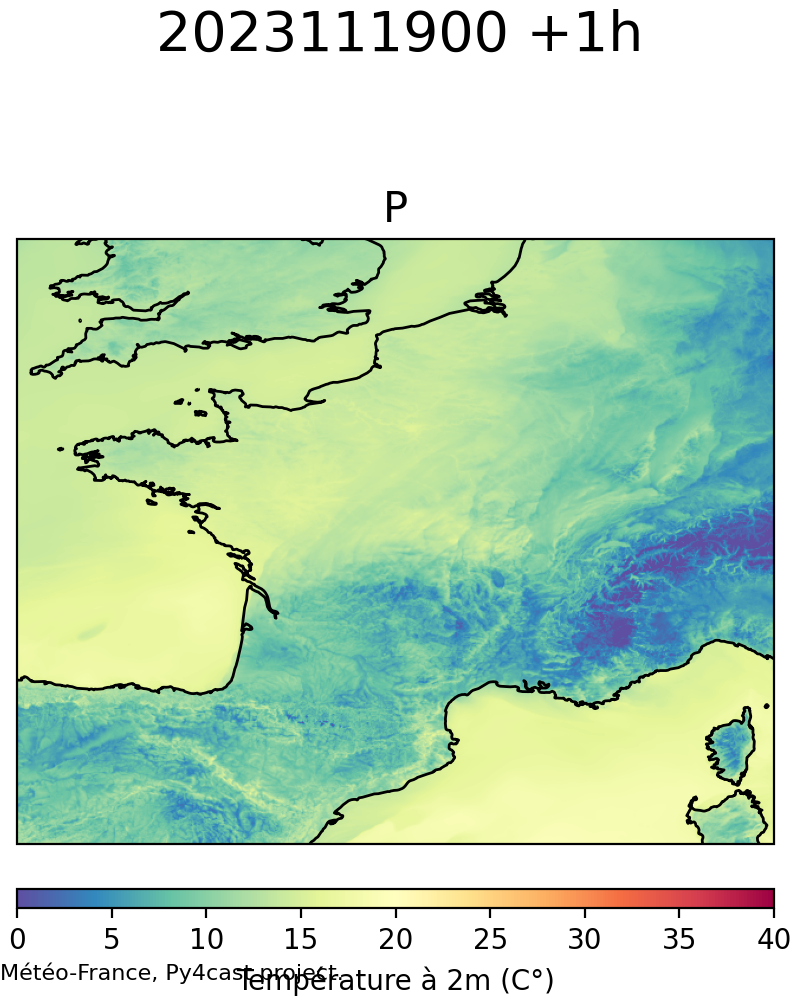
\includegraphics[width=0.2\textwidth]{Images/titan_data_examples/19_11/2023111900_feature_aro_t2m_2m.png}
        \hfill
        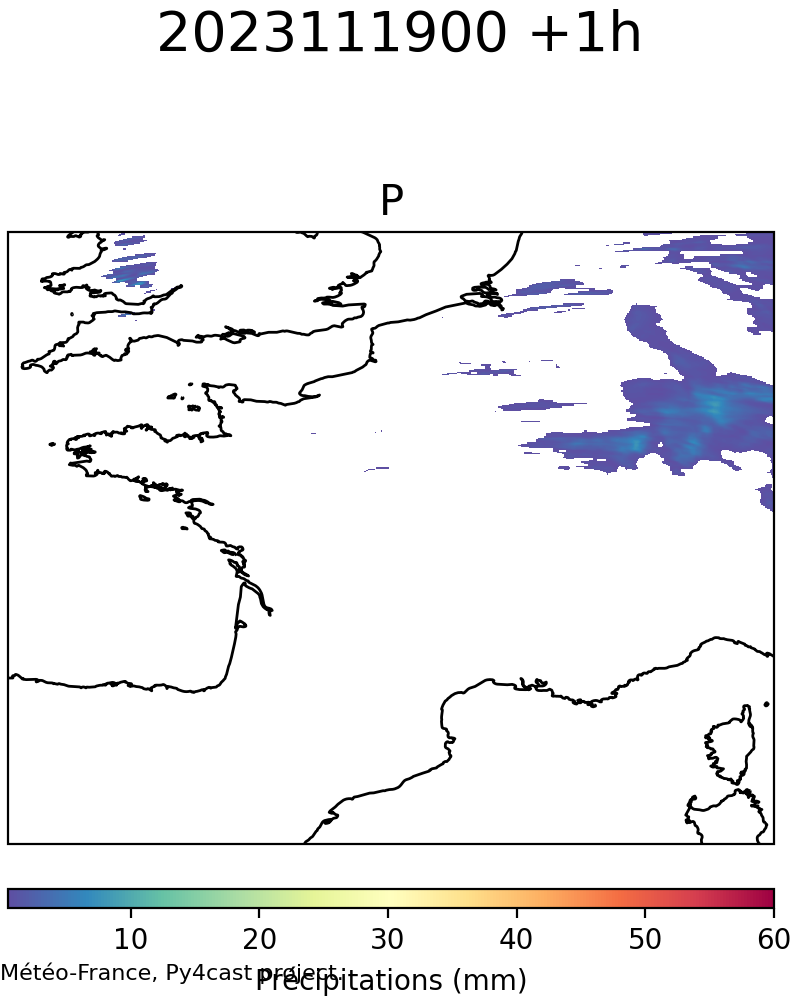
\includegraphics[width=0.2\textwidth]{Images/titan_data_examples/19_11/2023111900_feature_aro_tp_0m.png}
        \hfill
        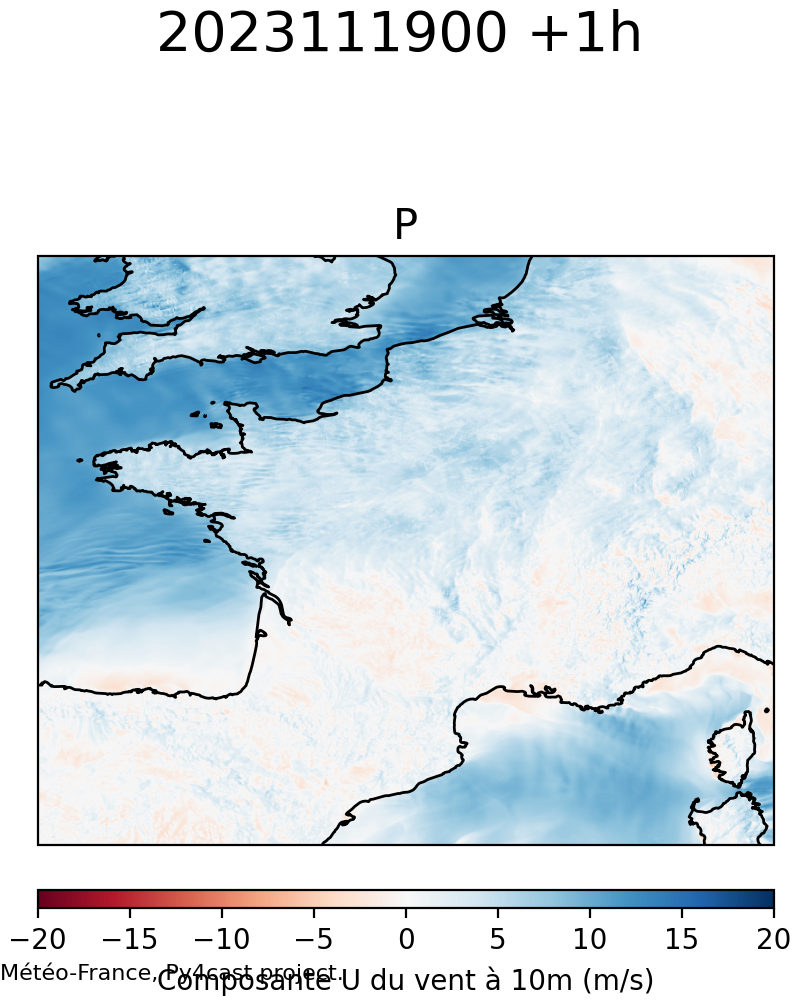
\includegraphics[width=0.2\textwidth]{Images/titan_data_examples/19_11/2023111900_feature_aro_u10_10m.png}
        \vfill
        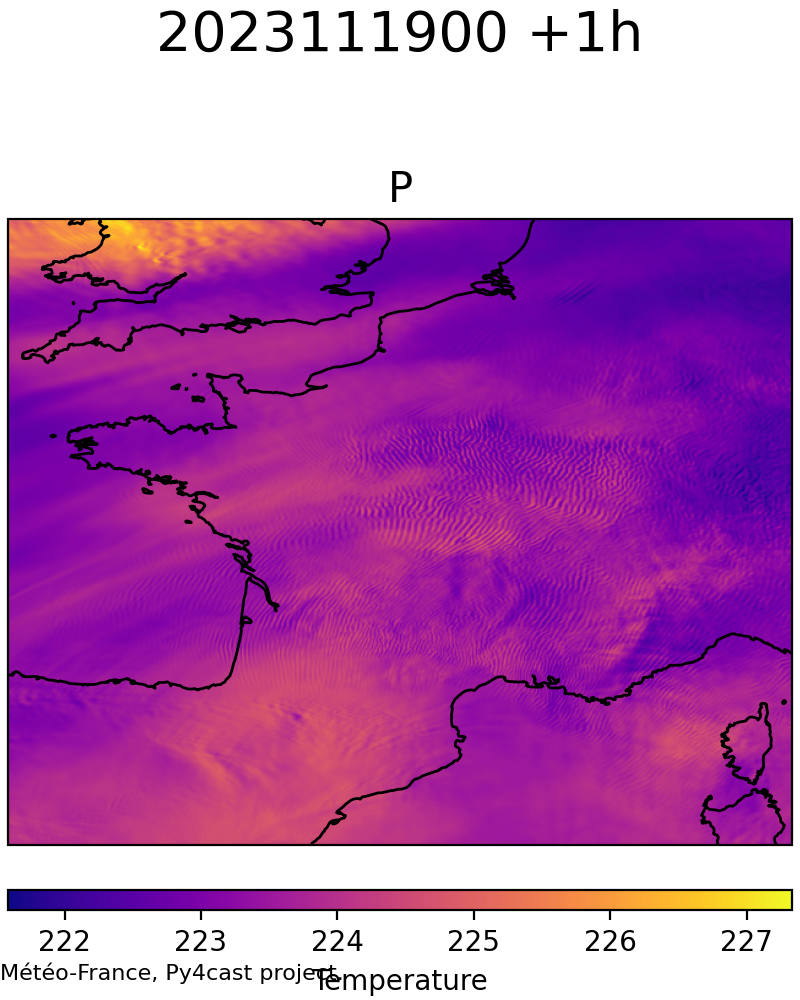
\includegraphics[width=0.2\textwidth]{Images/titan_data_examples/19_11/2023111900_feature_aro_t_250hpa.png}
        \hfill
        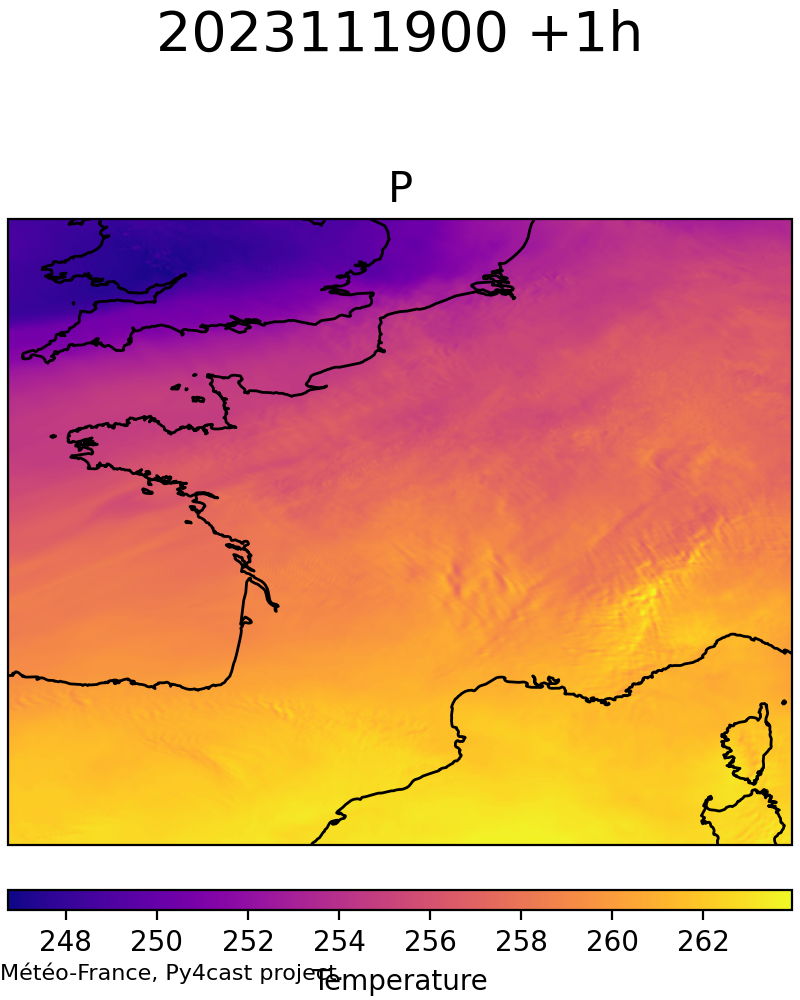
\includegraphics[width=0.2\textwidth]{Images/titan_data_examples/19_11/2023111900_feature_aro_t_500hpa.png}
        \hfill
        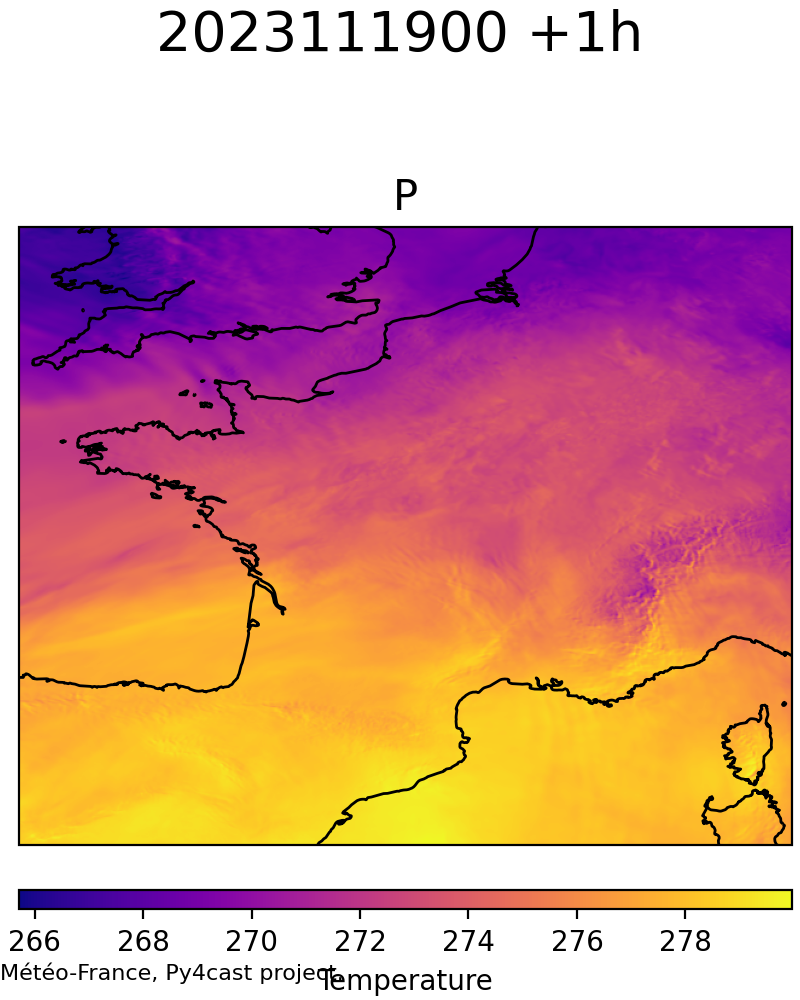
\includegraphics[width=0.2\textwidth]{Images/titan_data_examples/19_11/2023111900_feature_aro_t_700hpa.png}
        \hfill
        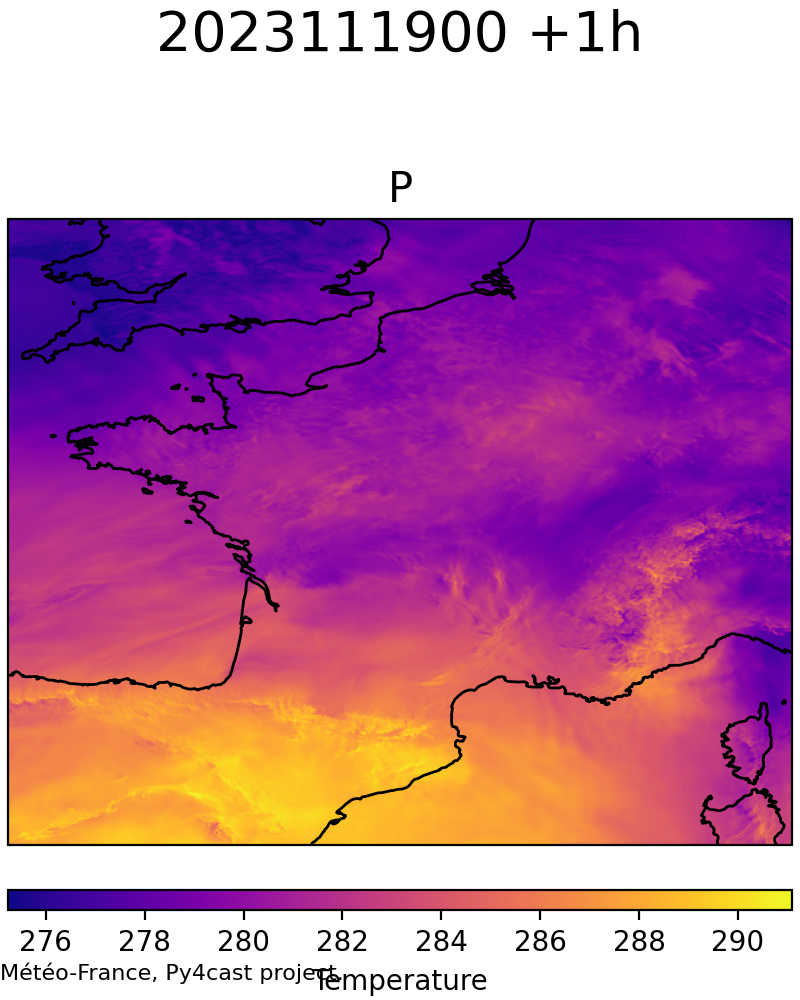
\includegraphics[width=0.2\textwidth]{Images/titan_data_examples/19_11/2023111900_feature_aro_t_850hpa.png}
        \caption{\scriptsize Titan image channels}
    \end{figure}
}{color3}

\subjectDevelopment{Combining AROME and ARPÈGE}{
Let $t$ be the present time and $t + 1$ be a future time.
\begin{itemize}
	\item Training without boundary conditions:
		\begin{itemize}
			\item Input: $aro_t$ (AROME at time $t$)
			\item Output: $aro_{t+1} - aro_t$ (The change in AROME from $t$ to $t+1$)
		\end{itemize}

	\item Training with boundary conditions:
		\begin{itemize}
			\item Input: $[aro_t, arp_t]$ (AROME and ARPÈGE at time $t$)
			\item Output: $aro_{t+1} - aro_t$ (The change in AROME from $t$ to $t+1$)
		\end{itemize}
\end{itemize}

In summary, the data can be combined in two primary ways: a simpler approach using only AROME data, and a more precise, operational-style approach that leverages \textbf{ARPÈGE data to provide essential boundary conditions}.
}{color3}

\subjectDevelopment{Py4cast Predictions}{
    \animategraphics[
        width=0.48\textwidth,
        autoplay,
        loop,
        palindrome
    ]{4}
    {Images/py4cast_predictions/frame_r2_}
    {001}
    {013}
    \hfill
    \animategraphics[
        width=0.48\textwidth,
        autoplay,
        loop,
        palindrome
    ]{4}
    {Images/py4cast_predictions/frame_tp_}
    {001}
    {013}
}{color3}

\subjectDevelopment{Applying Anchors on Weather Forecasting}{
We elaborated two extensions of the Anchors formalization, which will be particularly useful for the weather forecasting problem.

\begin{itemize}
	\item Deterministic Precision Constraint:

	\begin{equation}
		\arg \max_{A} {\text{cov}(A) \mid \text{prec}(A) \geq \tau }
		\label{eq:extended-max-cov-anchors}
	\end{equation}

	\item Extension to Regression and Probabilistic Output:
	
	\begin{equation}
		\text{prec}(A) = \mathbb{E}_{D(z|A)} [\mathbf{1}_{|f(x) - f(z)| > \tau}]
		\label{eq:extended-prec-anchors}
	\end{equation}

	where $\tau$ is a threshold above which the conditions of A are supposed to have a significant impact.
\end{itemize}
}{color3}

\subjectDevelopment{Generating data perturbations}{
    We suppose that $g_{i,j,c,R}(f(x_t)) == 1$, given a region $(i, j)$ in the map,  and we want to explain why using anchors. We will sample $K$ different counterfactual observations ${z_k}$, for $k \in {1, \ldots , K}$.

\begin{itemize}
	\item \textbf{Center of Perturbation:} $(\widehat{i_k}, \widehat{j_k})$
	
	\item \textbf{Channel of Perturbation:} $\widehat{c_k}$
	
	\item \textbf{Perturbation Value:} $\widehat{v_k}$
\end{itemize}
}{color3}

\subjectDevelopment{Perturbation Mask}{
    We introduce a second hyperparameter, $\sigma_e$, which models the spatial extent of the perturbation. The procedure for generating a counterfactual instance $z_k$ is then as follows:
\begin{itemize}
	\item \textbf{Unaffected Channels:} For all channels $c \neq \widehat{c_k}$, the data remains unchanged: $z_k(:, :, c) = x_t(:, :, c)$.
	
	\item \textbf{Mask Creation:} A mask $m \in \mathbb{R}^{I \times J}$ is generated. Its values are initially drawn from a 2D Gaussian distribution centered at $(\widehat{i_k}, \widehat{j_k})$ with covariance matrix $\begin{bmatrix} \sigma_e & 0 \ 0 & \sigma_e \end{bmatrix}$. These values are then linearly rescaled to the interval $[0, 1]$.
	
	\item \textbf{Application:} The perturbed channel $\widehat{c_k}$ in $z_k$ is created by a mask-based blending between the original values and the new value $\widehat{v_k}$:
	\begin{equation}
		z_k(\overline{i} , \overline{j} , \widehat{c_k}) = m(\overline{i} , \overline{j} ) * \widehat{v_k} + (1 - m(\overline{i} , \overline{j})) * x_t(\overline{i} , \overline{j}, \widehat{c_k})
		\label{eq:anchor-perturbation}
	\end{equation}
	for all $\overline{i} \in {1, \ldots, I}$ and $\overline{j} \in {1, \ldots, J}$.
\end{itemize}
}{color3}

\subjectDevelopment{Example of a Perturbed Image}{
\begin{figure}[h]
    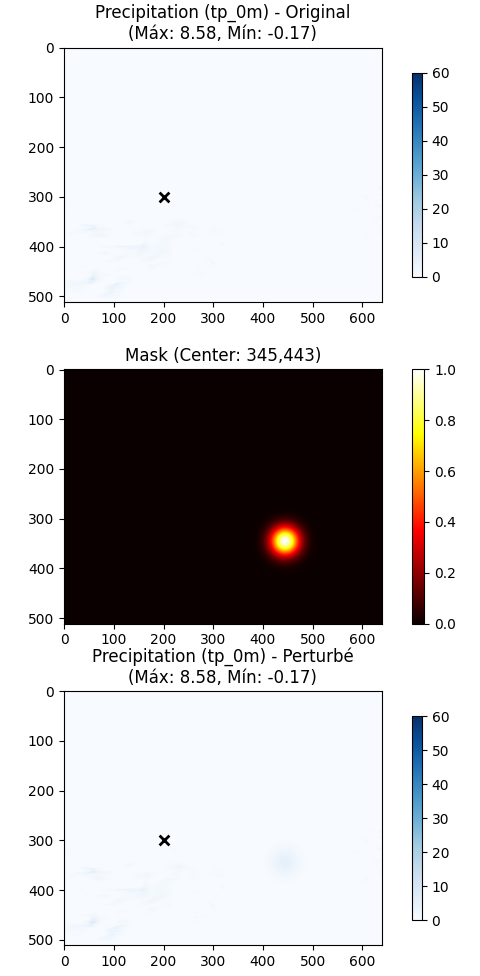
\includegraphics[width=0.3\textwidth]{Images/titan_rain_perturbations/perturbed_c_tp_0m.png}
    \hfill
    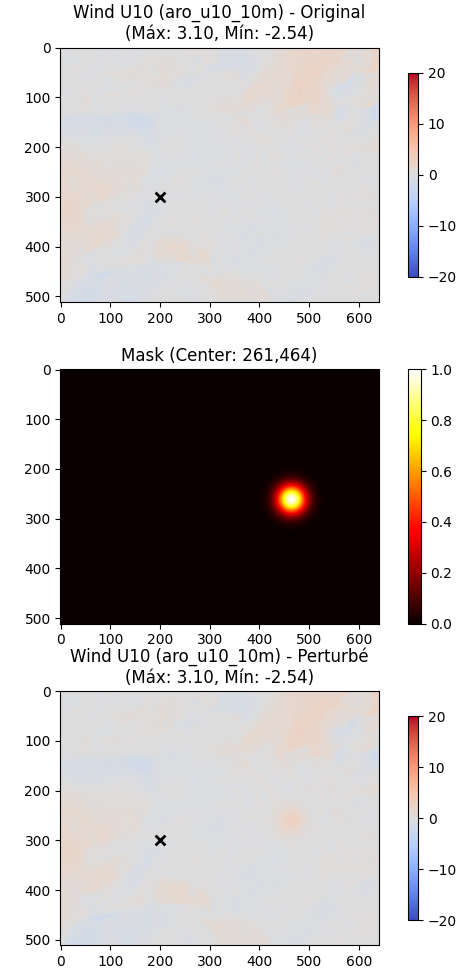
\includegraphics[width=0.3\textwidth]{Images/titan_rain_perturbations/perturbed_c_u10_10m.png}
    \hfill
    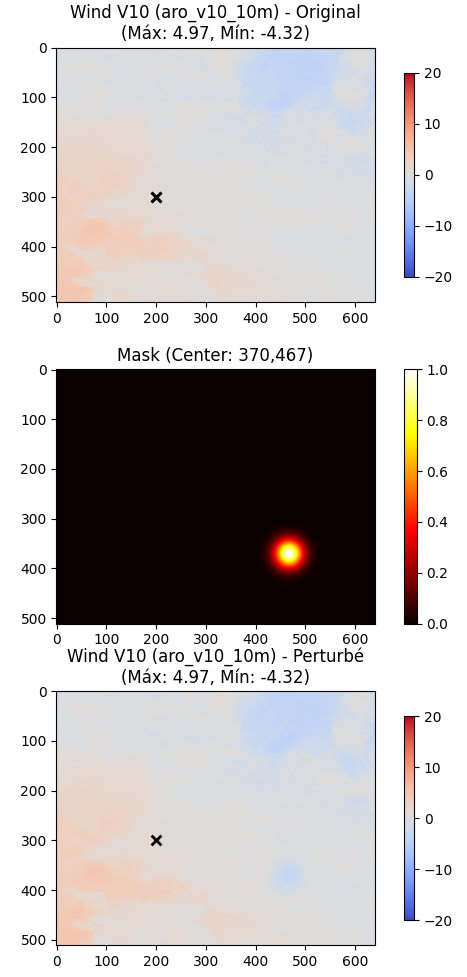
\includegraphics[width=0.3\textwidth]{Images/titan_rain_perturbations/perturbed_c_v10_10m.png}
    \caption{Example of counterfactuals of Titan image channels from 18/11/2023}
    \label{fig:titan-rain-perturbations}
\end{figure}
}{color3}

\subjectDevelopment{Running the Regression Anchors}{
    We generated about 300 conterfactuals per channel, in a radius of about \textbf{300 km from the target point}.
    \vfill
    Using a \textbf{mask of 40 km} for the perturbations.
    \vfill
    Seeing if the \textbf{rain prediction changed} in more than 5\%.
}{color3}

\subjectDevelopment{Rain Model}{
\begin{itemize}
    \item \textit{aro\_tp\_0m} (Total Precipitation)
	\item \textit{aro\_u10\_10m} (Zonal wind component at 10m)
    \item \textit{aro\_v10\_10m} (Meridional wind component at 10m)
\end{itemize}
}{color3}

\subjectDevelopment{Region of Chateaubriant on $18^{th}$ November}{
\begin{figure}[h]
    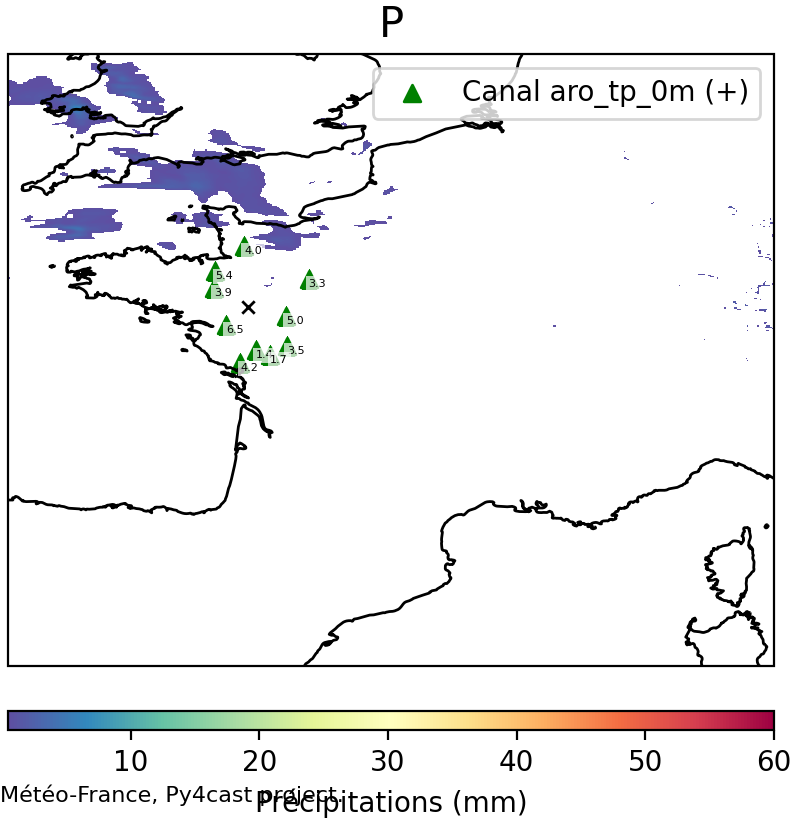
\includegraphics[width=0.38\textwidth]{Images/titan_rain_anchors/nov-18/2023111800_feature_aro_tp_0m.png}
    \hfill
    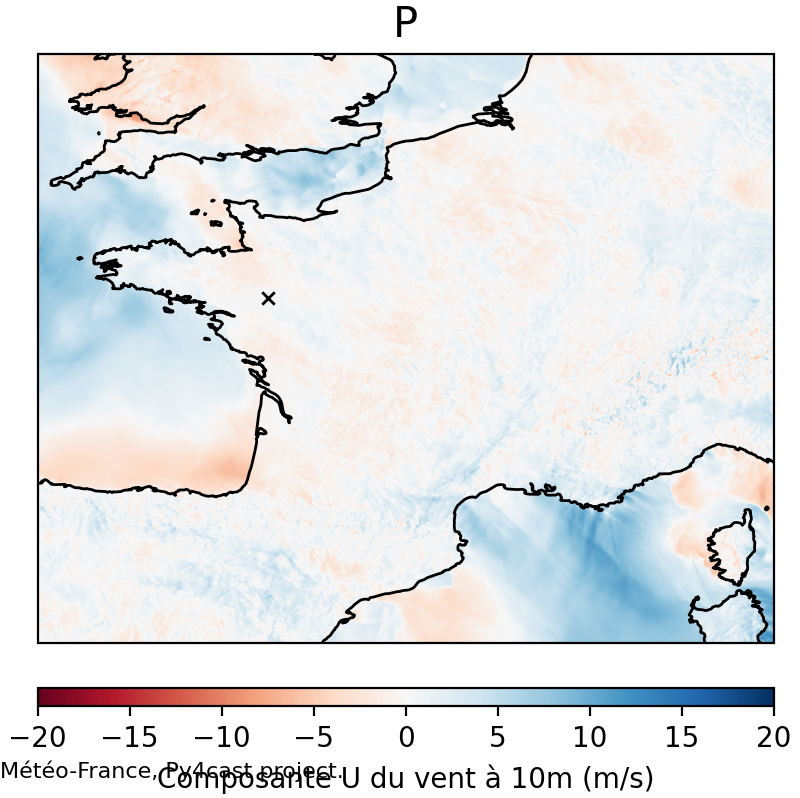
\includegraphics[width=0.38\textwidth]{Images/titan_rain_anchors/nov-18/2023111800_feature_aro_u10_10m.png}
    \hfill
    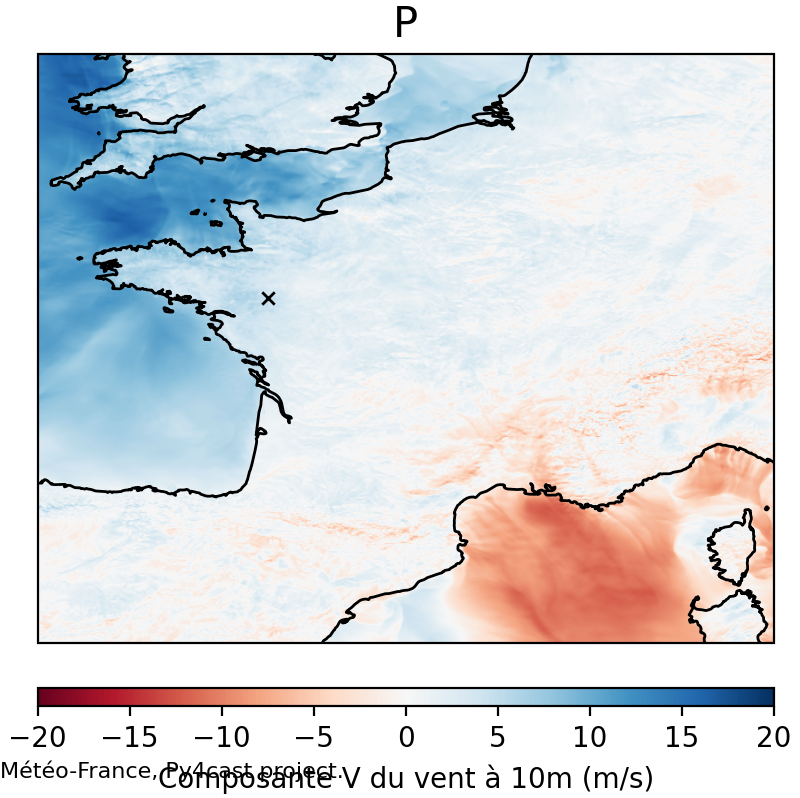
\includegraphics[width=0.38\textwidth]{Images/titan_rain_anchors/nov-18/2023111800_feature_aro_v10_10m.png}
\end{figure}
}{color3}

\subjectDevelopment{Region of Limoges on $21^{st}$ November}{
\begin{figure}[h]
    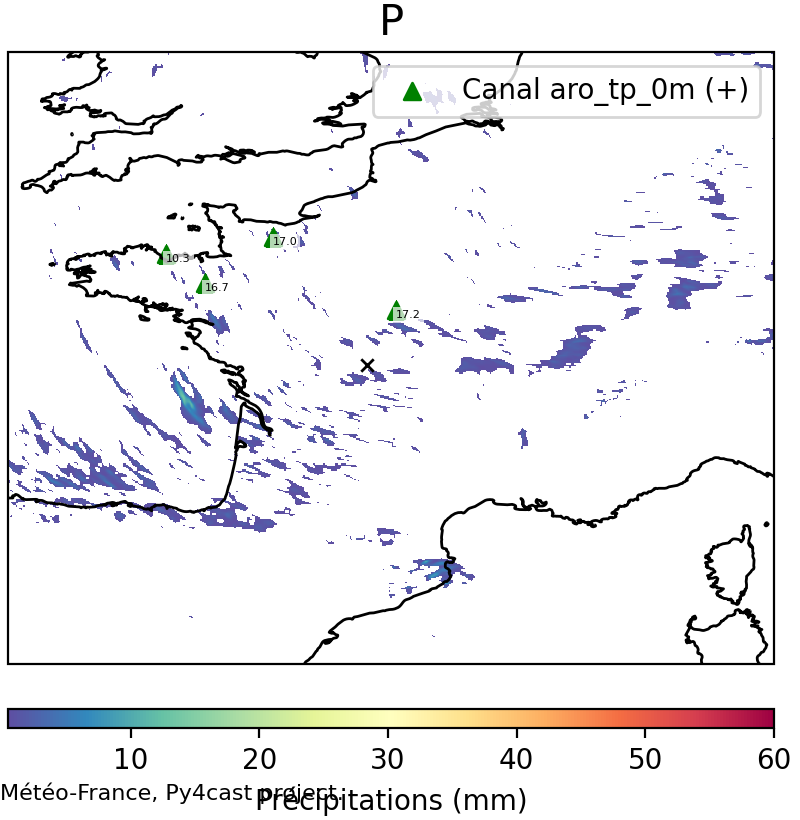
\includegraphics[width=0.38\textwidth]{Images/titan_rain_anchors/nov-21/2023112100_feature_aro_tp_0m.png}
    \hfill
    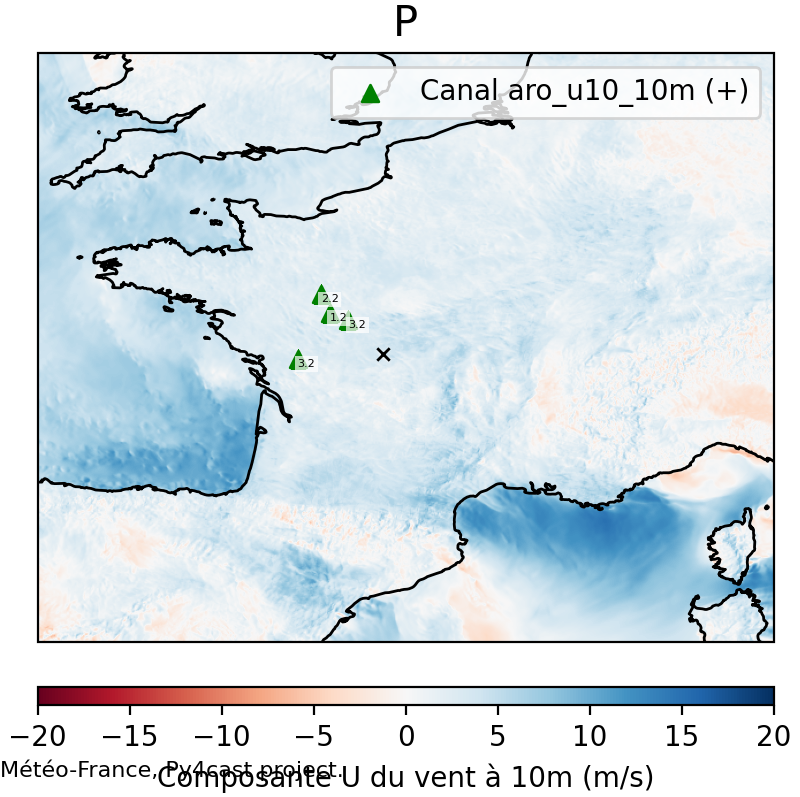
\includegraphics[width=0.38\textwidth]{Images/titan_rain_anchors/nov-21/2023112100_feature_aro_u10_10m.png}
    \hfill
    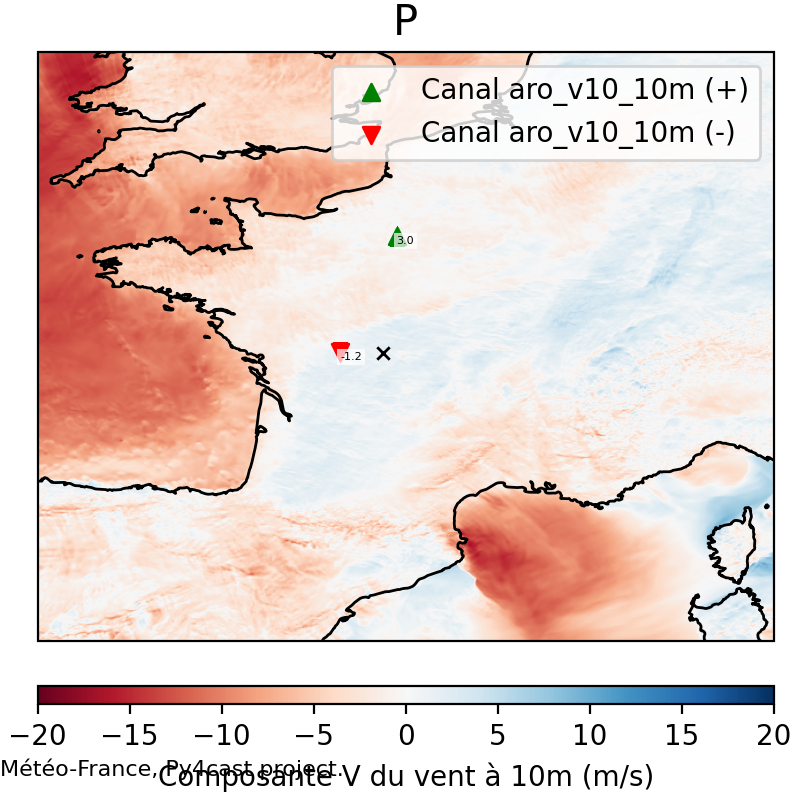
\includegraphics[width=0.38\textwidth]{Images/titan_rain_anchors/nov-21/2023112100_feature_aro_v10_10m.png}
    \caption{Example of anchors applied on "rain" channels, on $21^{st}$ November data.}
    \label{fig:titan-rain-anchors-21}
\end{figure}
}{color3}

\subjectPresentation{4}{Results}{color4}

\subjectDevelopment{Different Models to Compare}{
\begin{enumerate}
    \item \textbf{Rain Model (No Boundaries):} Trained exclusively on the three AROME rain channels, as presented in the previous results.
    \item \textbf{Rain Model (With Boundaries):} Trained on the three AROME rain channels augmented with all ARPÈGE global fields as boundary conditions.
    \item \textbf{Full Model (No Boundaries):} Trained on the complete set of 21 AROME channels, without boundary conditions.
    \item \textbf{Full Model (With Boundaries):} Trained on the full suite of AROME channels combined with all ARPÈGE global fields to provide boundary conditions.
\end{enumerate}
}{color4}

\subjectDevelopment{Rain Model With Boundaries}{
\begin{figure}[h]
    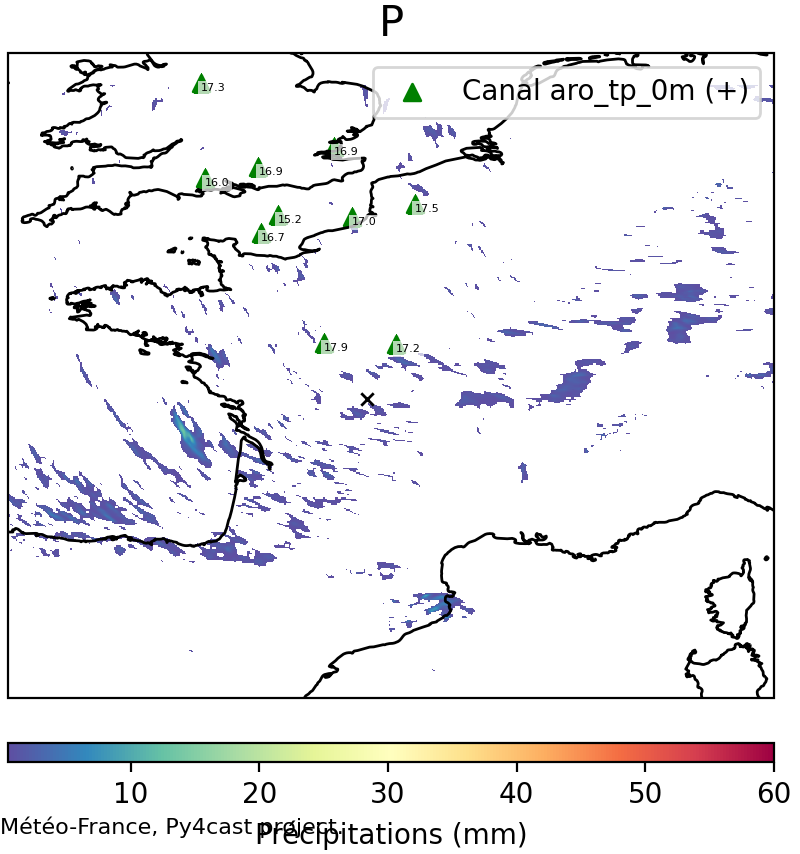
\includegraphics[width=0.38\textwidth]{Images/titan_rain_anchors/nov-21/rain-arp/2023112100_feature_aro_tp_0m.png}
    \hfill
    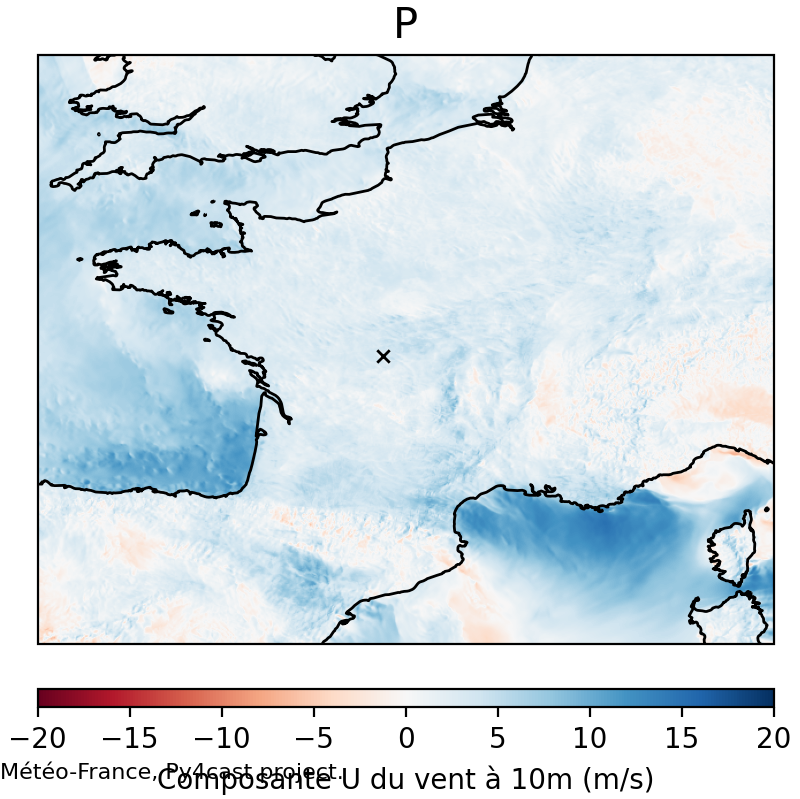
\includegraphics[width=0.38\textwidth]{Images/titan_rain_anchors/nov-21/rain-arp/2023112100_feature_aro_u10_10m.png}    
    \hfill
    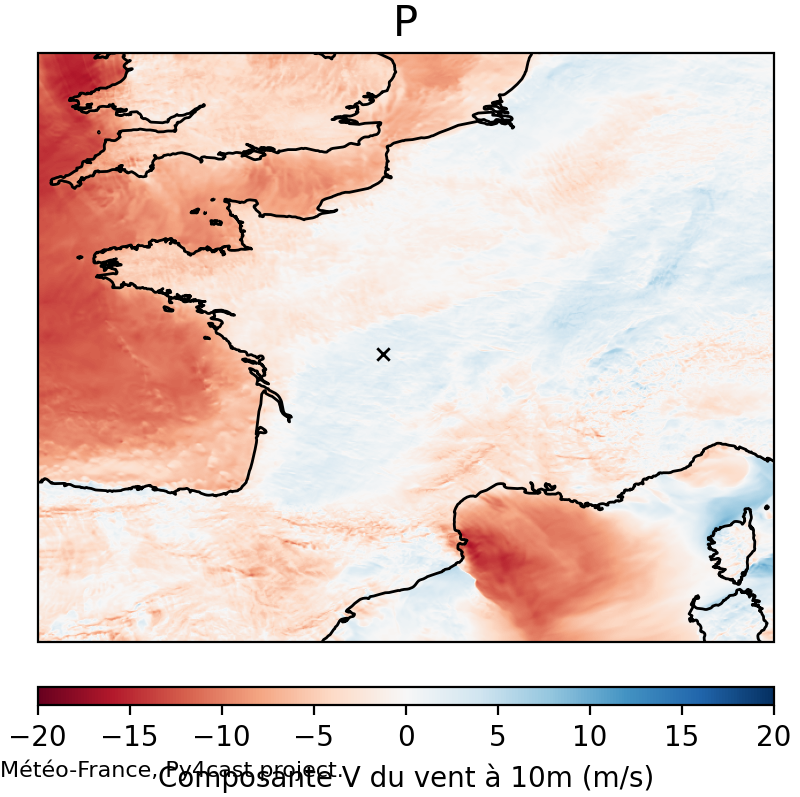
\includegraphics[width=0.38\textwidth]{Images/titan_rain_anchors/nov-21/rain-arp/2023112100_feature_aro_v10_10m.png}    
    \label{fig:titan-rain-arp-anchors-21}
\end{figure}
}{color4}

\subjectDevelopment{Full Model Without Boundaries}{
\begin{figure}[h]
    \centering
    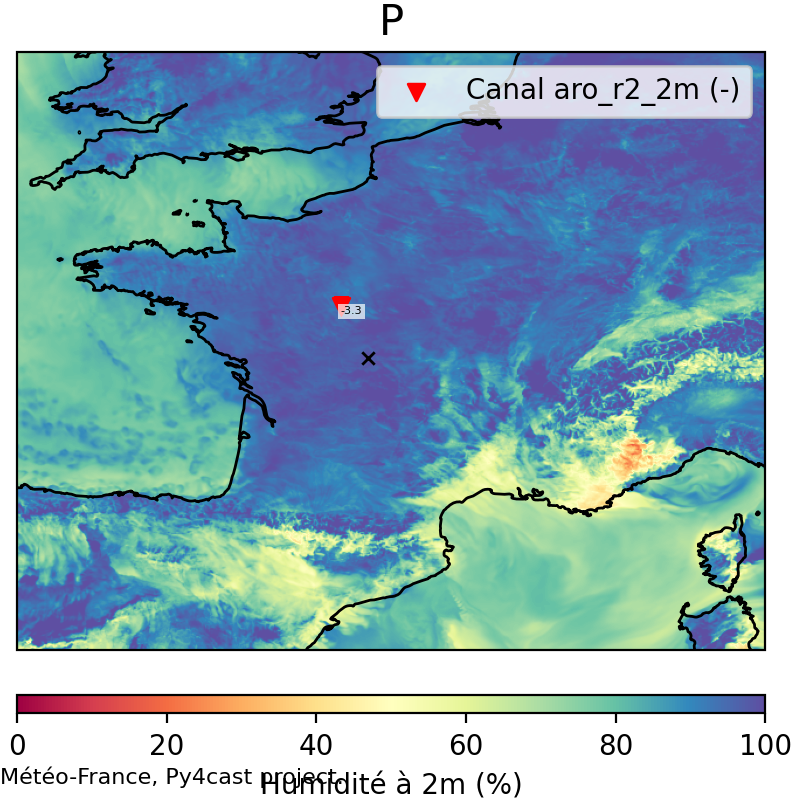
\includegraphics[width=0.38\textwidth]{Images/titan_rain_anchors/nov-21/complete/2023112100_feature_aro_r2_2m.png}
    \hfill
    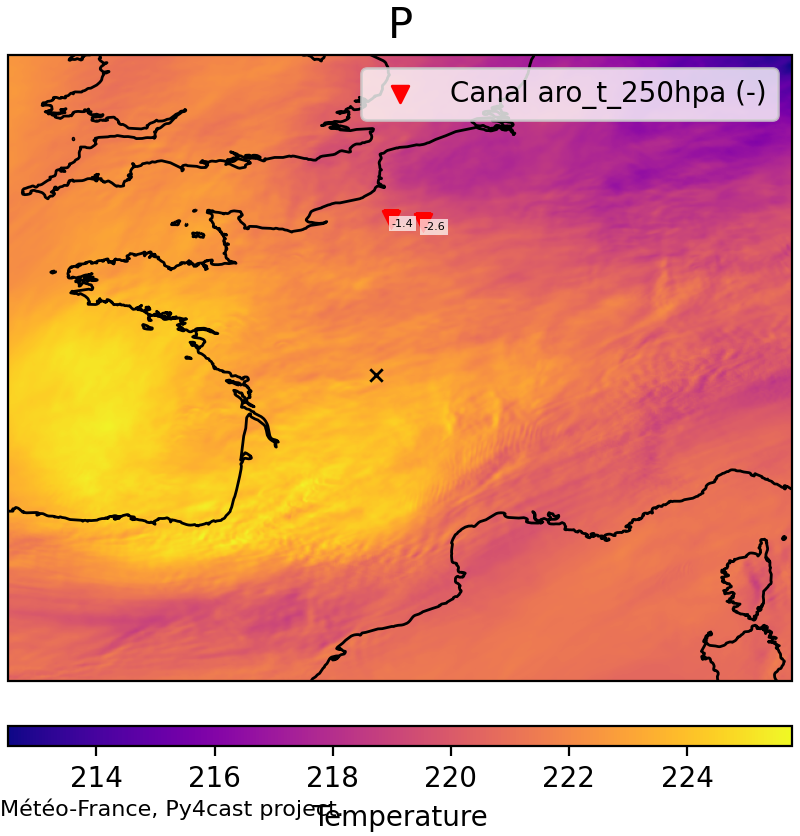
\includegraphics[width=0.38\textwidth]{Images/titan_rain_anchors/nov-21/complete/2023112100_feature_aro_t_250hpa.png}
    \hfill
    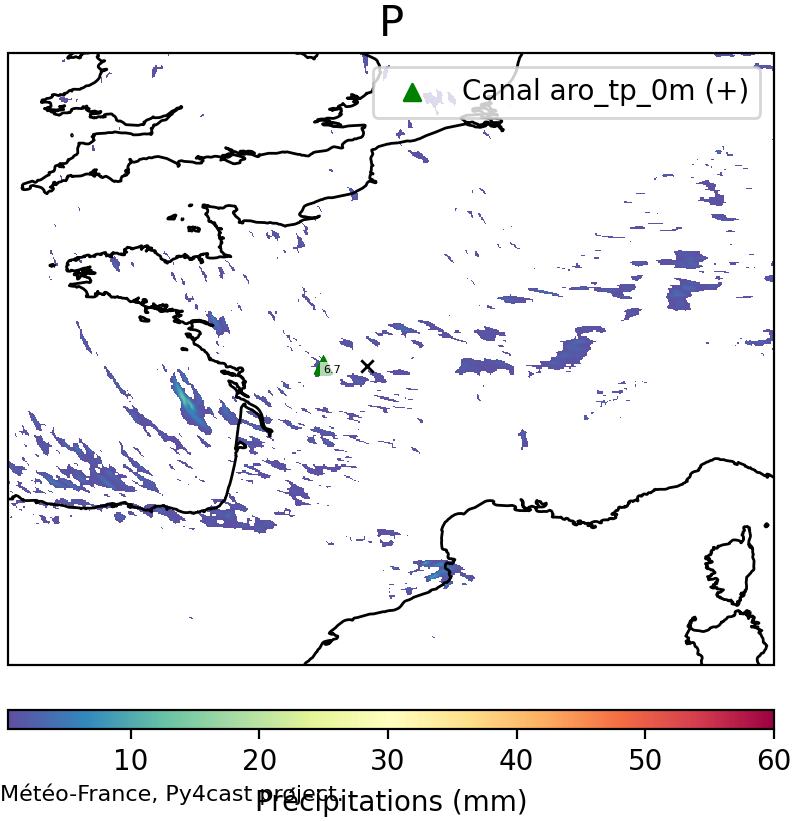
\includegraphics[width=0.38\textwidth]{Images/titan_rain_anchors/nov-21/complete/2023112100_feature_aro_tp_0m.png}
    \hfill
    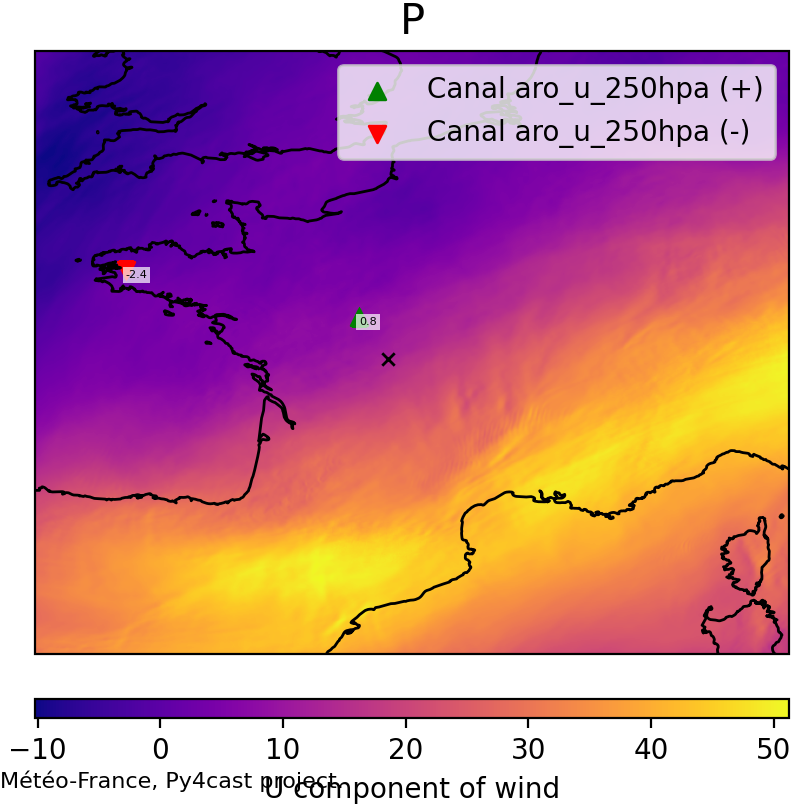
\includegraphics[width=0.38\textwidth]{Images/titan_rain_anchors/nov-21/complete/2023112100_feature_aro_u_250hpa.png}
\end{figure}
}{color4}

\subjectDevelopment{Full Model Without Boundaries}{
\begin{figure}[h]
    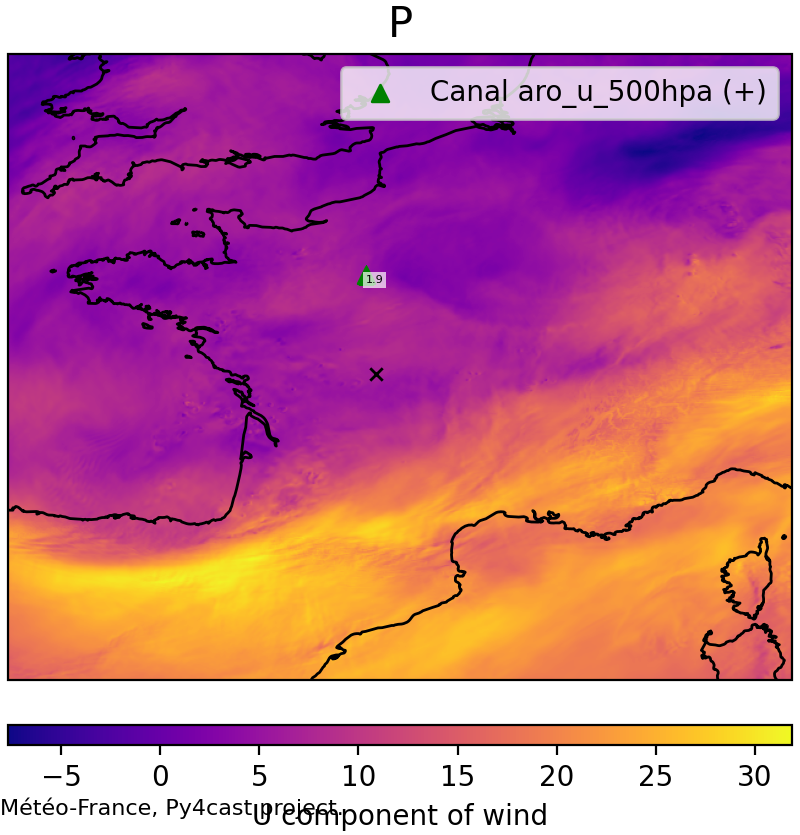
\includegraphics[width=0.38\textwidth]{Images/titan_rain_anchors/nov-21/complete/2023112100_feature_aro_u_500hpa.png}
    \hfill
    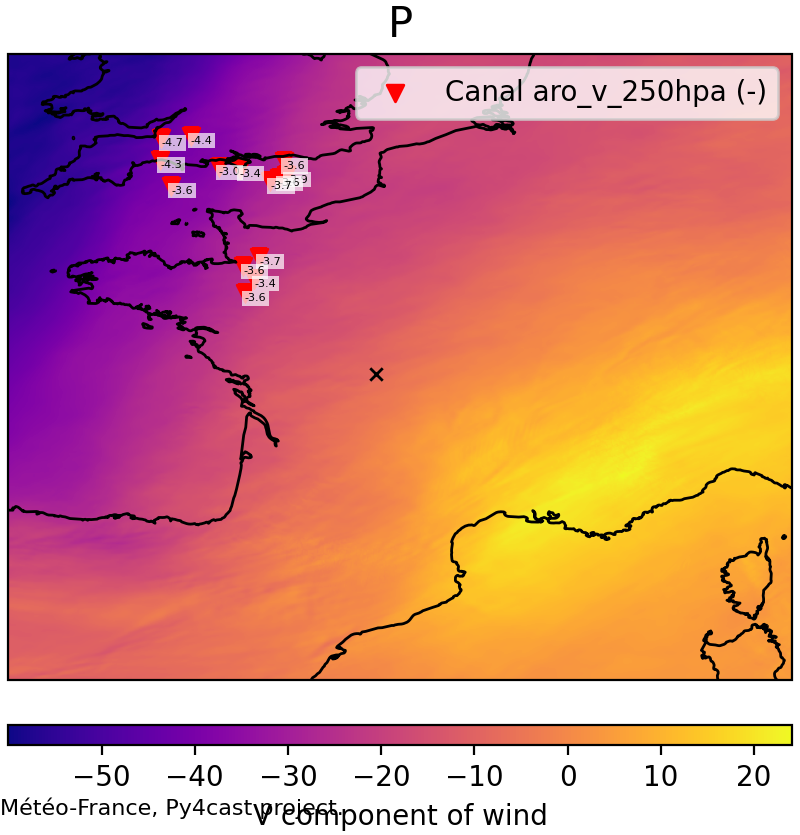
\includegraphics[width=0.38\textwidth]{Images/titan_rain_anchors/nov-21/complete/2023112100_feature_aro_v_250hpa.png}
    \hfill
    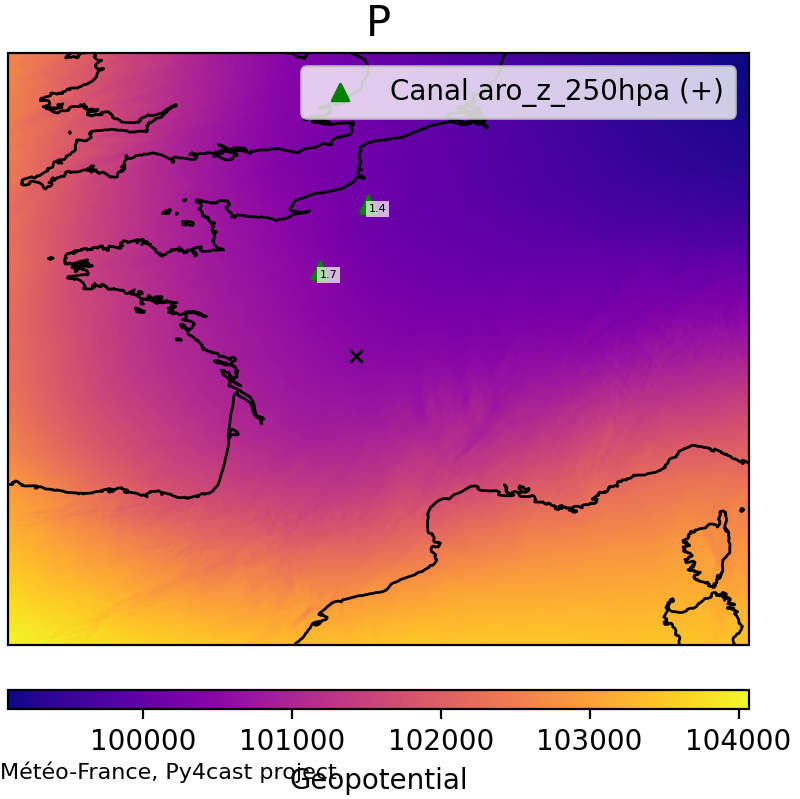
\includegraphics[width=0.38\textwidth]{Images/titan_rain_anchors/nov-21/complete/2023112100_feature_aro_z_250hpa.png}
    \hfill
    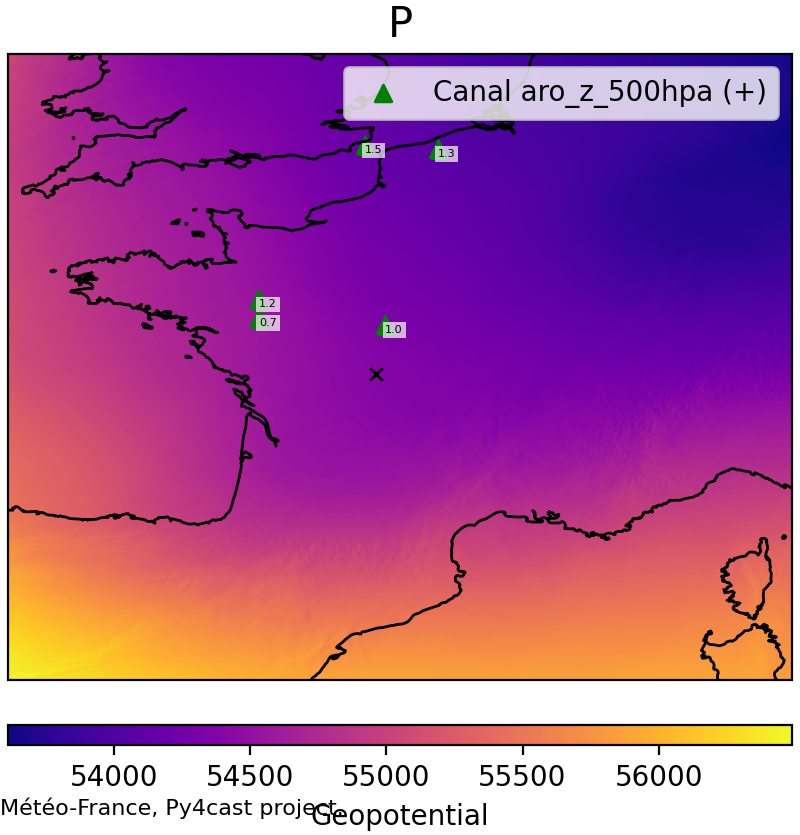
\includegraphics[width=0.38\textwidth]{Images/titan_rain_anchors/nov-21/complete/2023112100_feature_aro_z_500hpa.png}  
\end{figure}
}{color4}

\subjectDevelopment{Full Model Without Boundaries}{
\begin{figure}[h]
    \includegraphics[width=0.38\textwidth]{Images/titan_rain_anchors/nov-21/complete/2023112100_feature_aro_z_700hpa.png}
    \hfill
    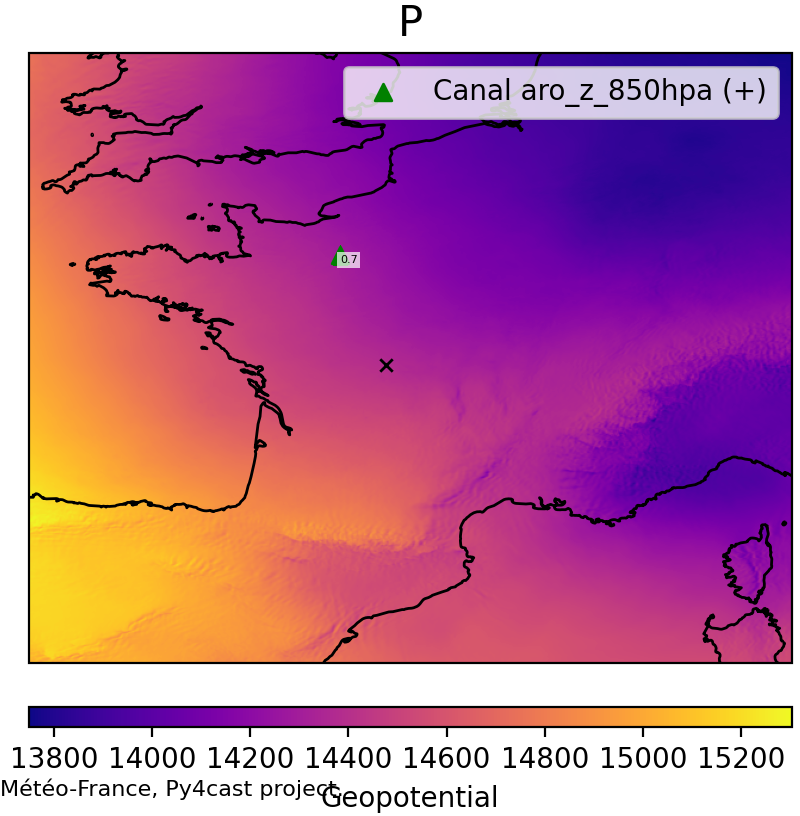
\includegraphics[width=0.38\textwidth]{Images/titan_rain_anchors/nov-21/complete/2023112100_feature_aro_z_850hpa.png}    
    \label{fig:titan-full-anchors-21}
\end{figure}
}{color4}

\subjectDevelopment{Full Model With Boundaries}{
\begin{figure}[h]
    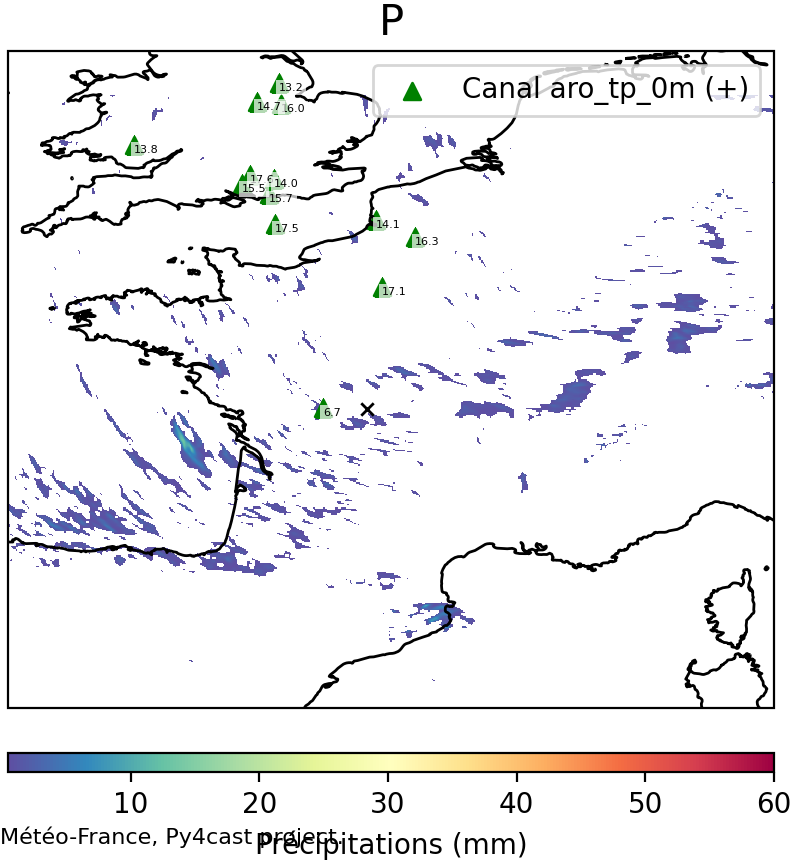
\includegraphics[width=0.38\textwidth]{Images/titan_rain_anchors/nov-21/complete-arp/2023112100_feature_aro_tp_0m.png}
    \hfill
    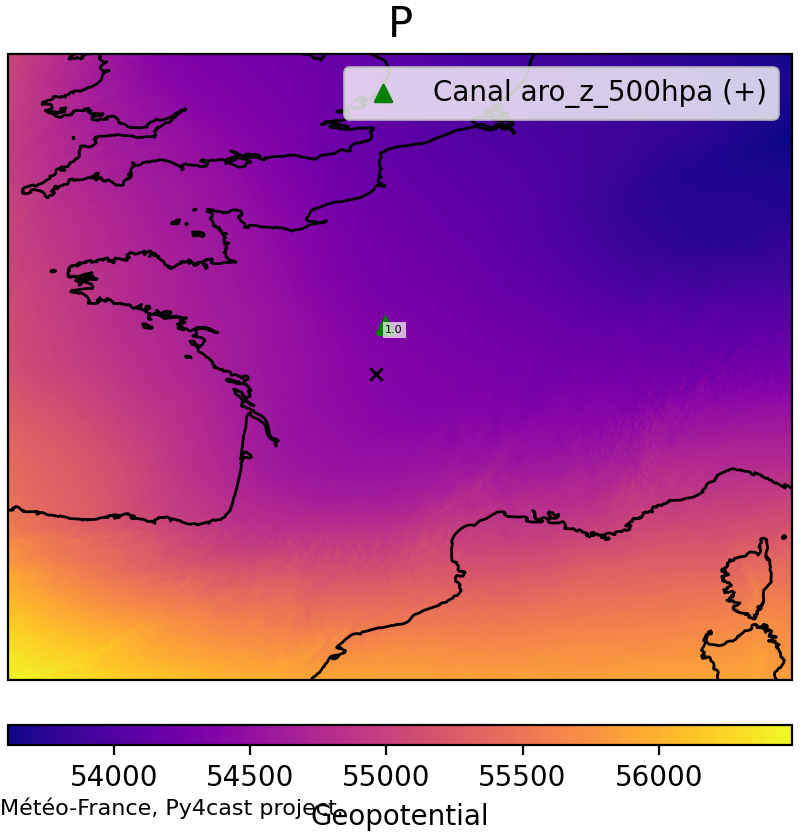
\includegraphics[width=0.38\textwidth]{Images/titan_rain_anchors/nov-21/complete-arp/2023112100_feature_aro_z_500hpa.png}
    \hfill
    \includegraphics[width=0.38\textwidth]{Images/titan_rain_anchors/nov-21/complete-arp/2023112100_feature_aro_z_700hpa.png}
    \label{fig:titan-full-arp-anchors-21}
\end{figure}
}{color4}

\subjectPresentation{5}{Discussion}{color5}

\subjectDevelopment{Some remarks on the Regression Anchors}{
The results for the Full Model without Boundaries can be interpreted by considering two factors: the number of anchors per channel (indicating influence) and the magnitude of their effect on the prediction.

\begin{itemize}
    \item Full Model with Boundaries reveals that the model trained with ARPÈGE data produced \textbf{more conservative and robust explanations}.
    \item It generated anchors in \textbf{fewer channels and with a lower density per channel}.
    \item  This increased selectivity may be due to the robustness introduced by the \textbf{global context provided by the ARPÈGE boundary conditions}.
    \item Despite this difference, there is an intersection between the anchors found in both models, indicating agreement on the importance of certain channels and locations.
\end{itemize}
}{color5}

\subjectPresentation{6}{Conclusion}{color6}

\subjectDevelopment{Insights on the Meteo}{
Furthermore, the method demonstrated potential to:
\begin{itemize}
    \item Understand the constraints used by the model for the prediction
    \item Proactive vulnerability mapping
    \item Highlighting surrounding areas that \textbf{highly influence a target location}, Anchors can reveal geographic points of sensitivity
\end{itemize}
That lead us to identify zones where extreme weather events elsewhere could have a critical downstream impact, thereby improving risk assessment and resource allocation.
}{color6}

\begin{frame}[plain]
  \begin{tikzpicture}[remember picture,overlay]
    \node at (current page){
\includegraphics[height=1\paperheight, keepaspectratio]{Images/background_ensta.png}};
  \end{tikzpicture}
  \vspace*{1cm}
  \centering
  
  \vfill
  
  Merci!
  
  \vfill
\end{frame}

\end{document}